\section{Iteración IX}
\subsection{Resumen}
Esta iteración es la integración de lo desarrollado en la iteración VIII (gestión de muebles y categorías en plataforma) a la iteración VII (gestión de escenarios). Además se hicieron mejoras en la usabilidad de la aplicación.

\subsection{Desarrollo}
En la iteración VII usamos modelos y categorías estáticos para realizar las pruebas de funcionalidad.\par
Las categorías y subcategorías gestionadas por el usuario en la plataforma web se muestran én el menú de muebles (ver figura 4.63). Asimismo teniendo los muebles ya almacenados en la plataforma web en la iteración anterior, desarrollamos un proceso para poder obtener de AWS S3 (lugar donde se encuentran almacenados todos los modelos subidos) los muebles subidos previamente y su imagen para mostrarlos en el menú de muebles de forma dinámica (ver figura 4.64), de tal forma que estos puedan ser utilizados en la construcción de escenarios (ver figura 4.65).


\begin{figure}[h!]
	\begin{minipage}{0.32\textwidth}
		\centering
		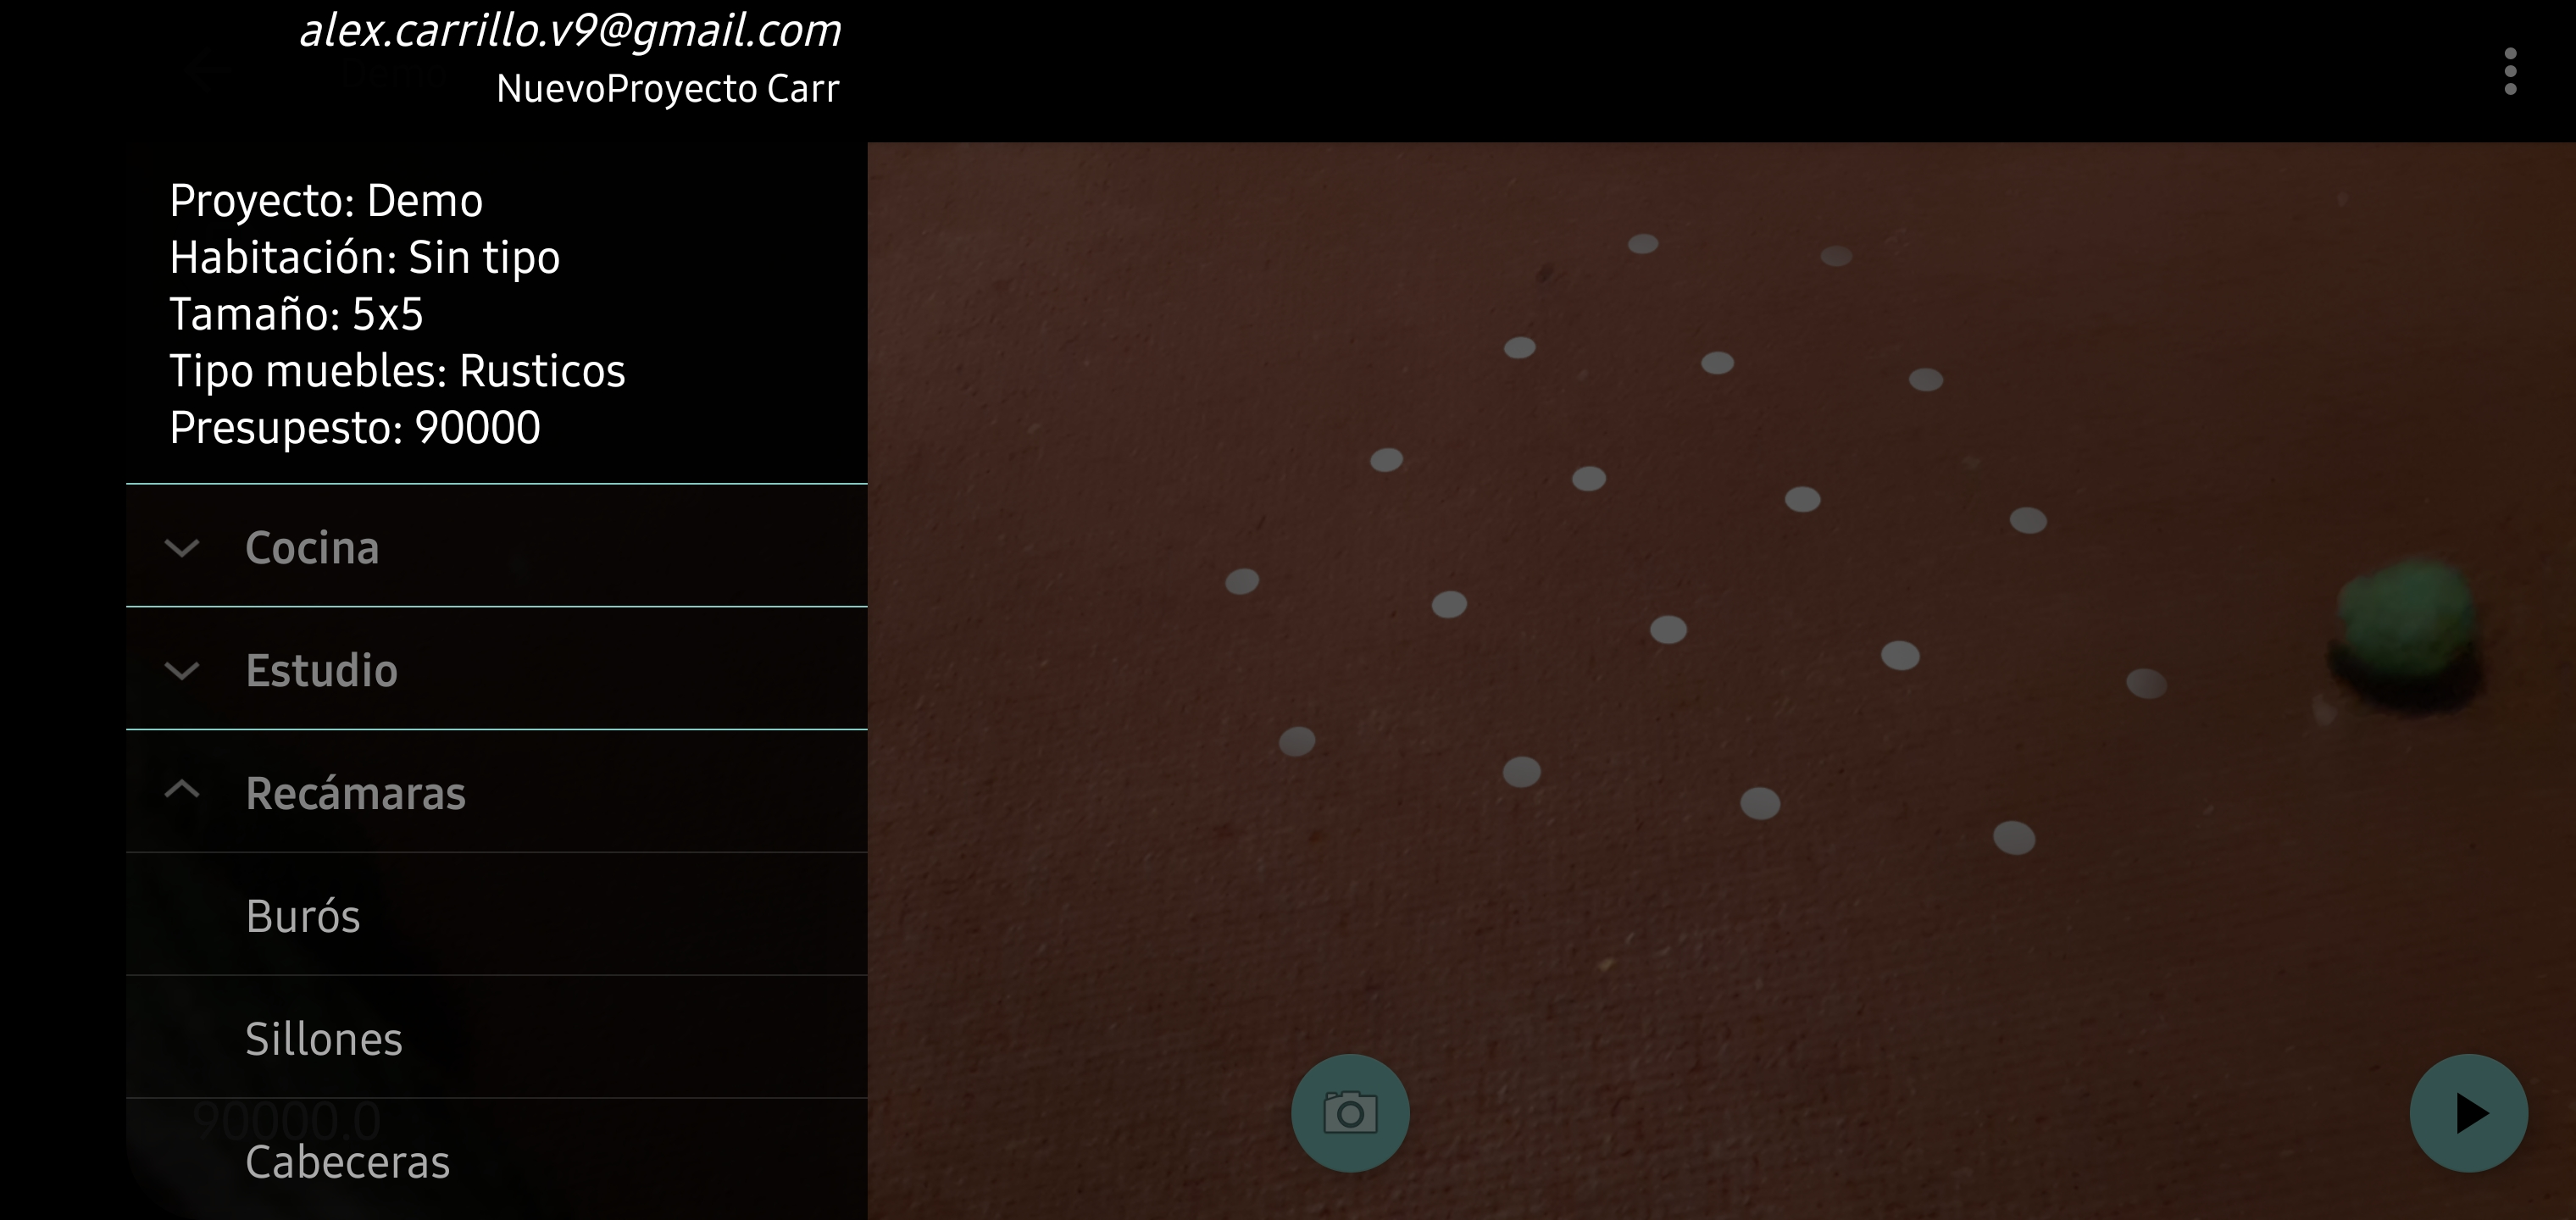
\includegraphics[width=4cm,height=8cm]{imagenes/desarrollo/app/categories.jpg}
		\caption{Categorías y subcategorías de usuario.}
		\label{fig:appmenucat}
	\end{minipage}\hfill
	\begin{minipage}{0.32\textwidth}
		\centering
		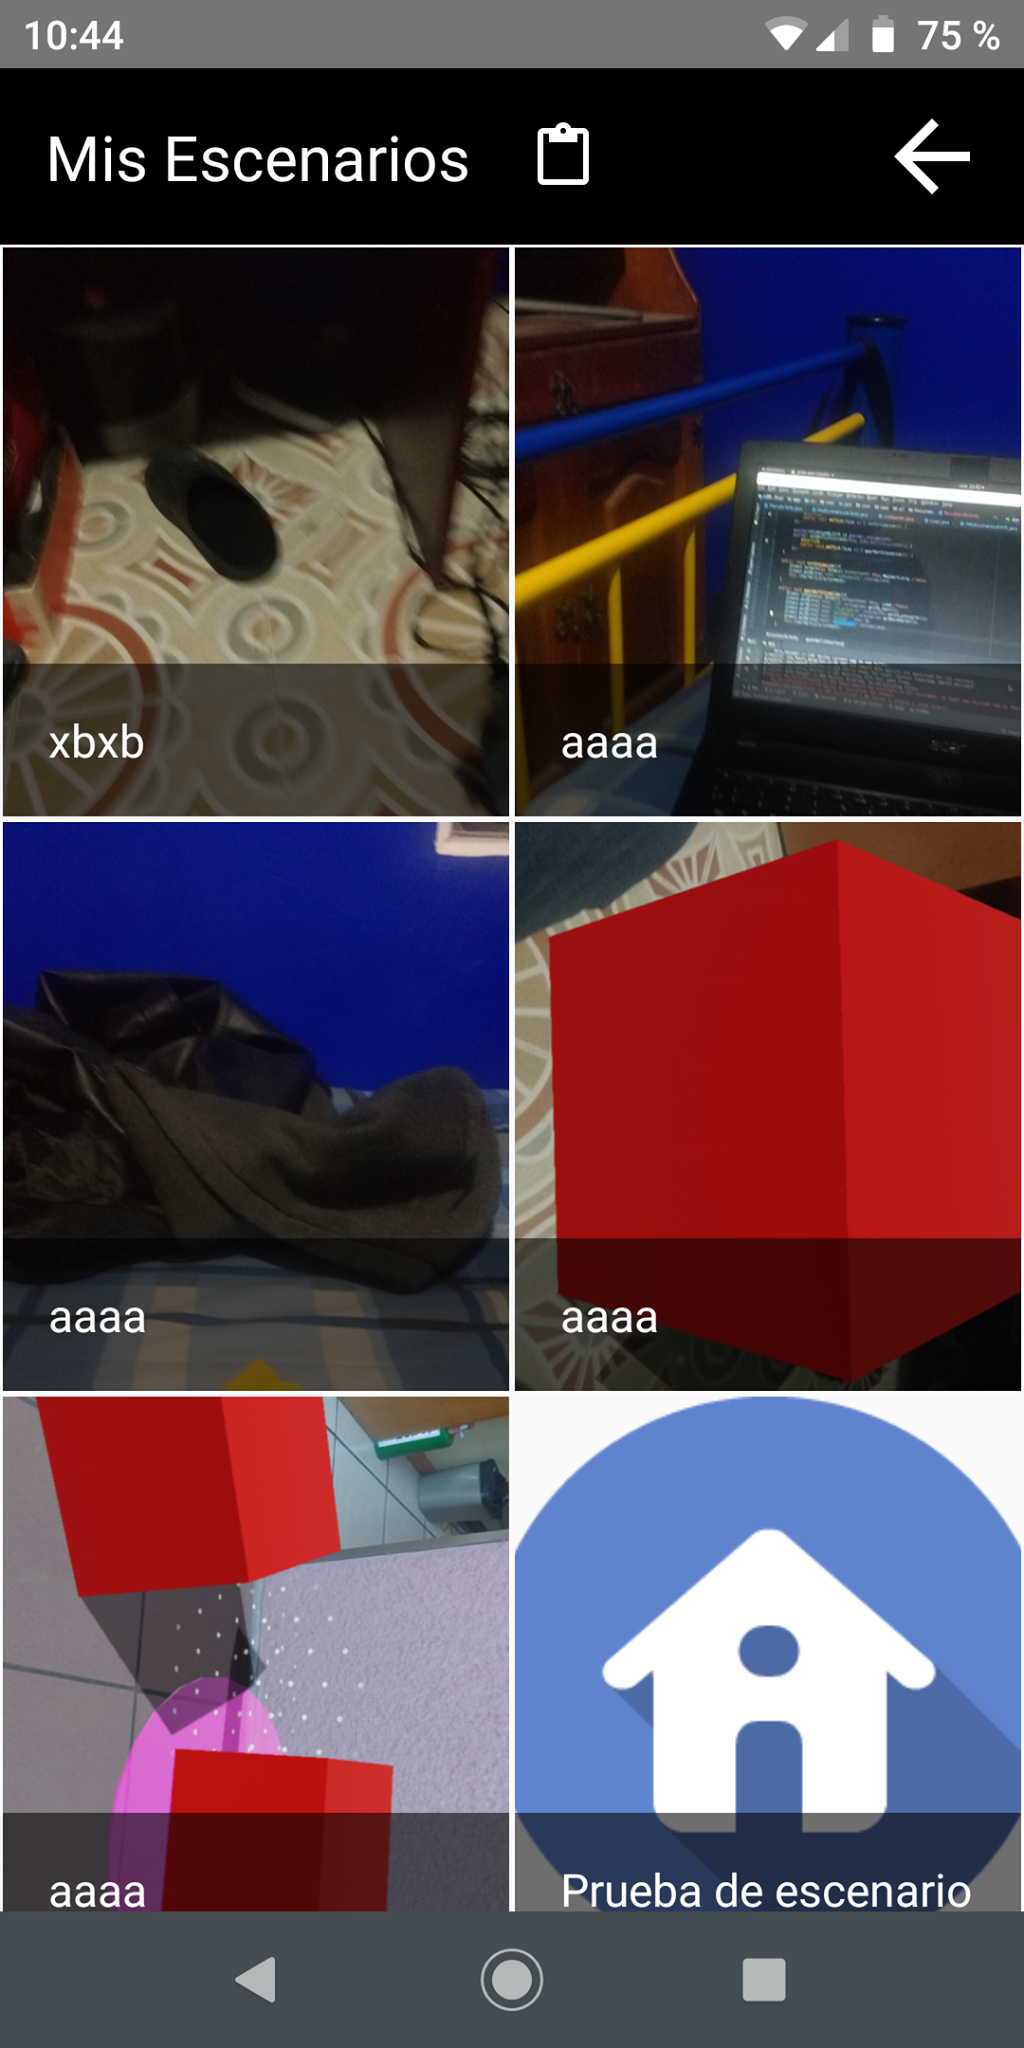
\includegraphics[width=4cm,height=8cm]{imagenes/desarrollo/app/scenarios.png}
		\caption{Menú de muebles}
		\label{fig:appmenu}
	\end{minipage}\hfill
	\begin{minipage}{0.32\textwidth}
		\centering
		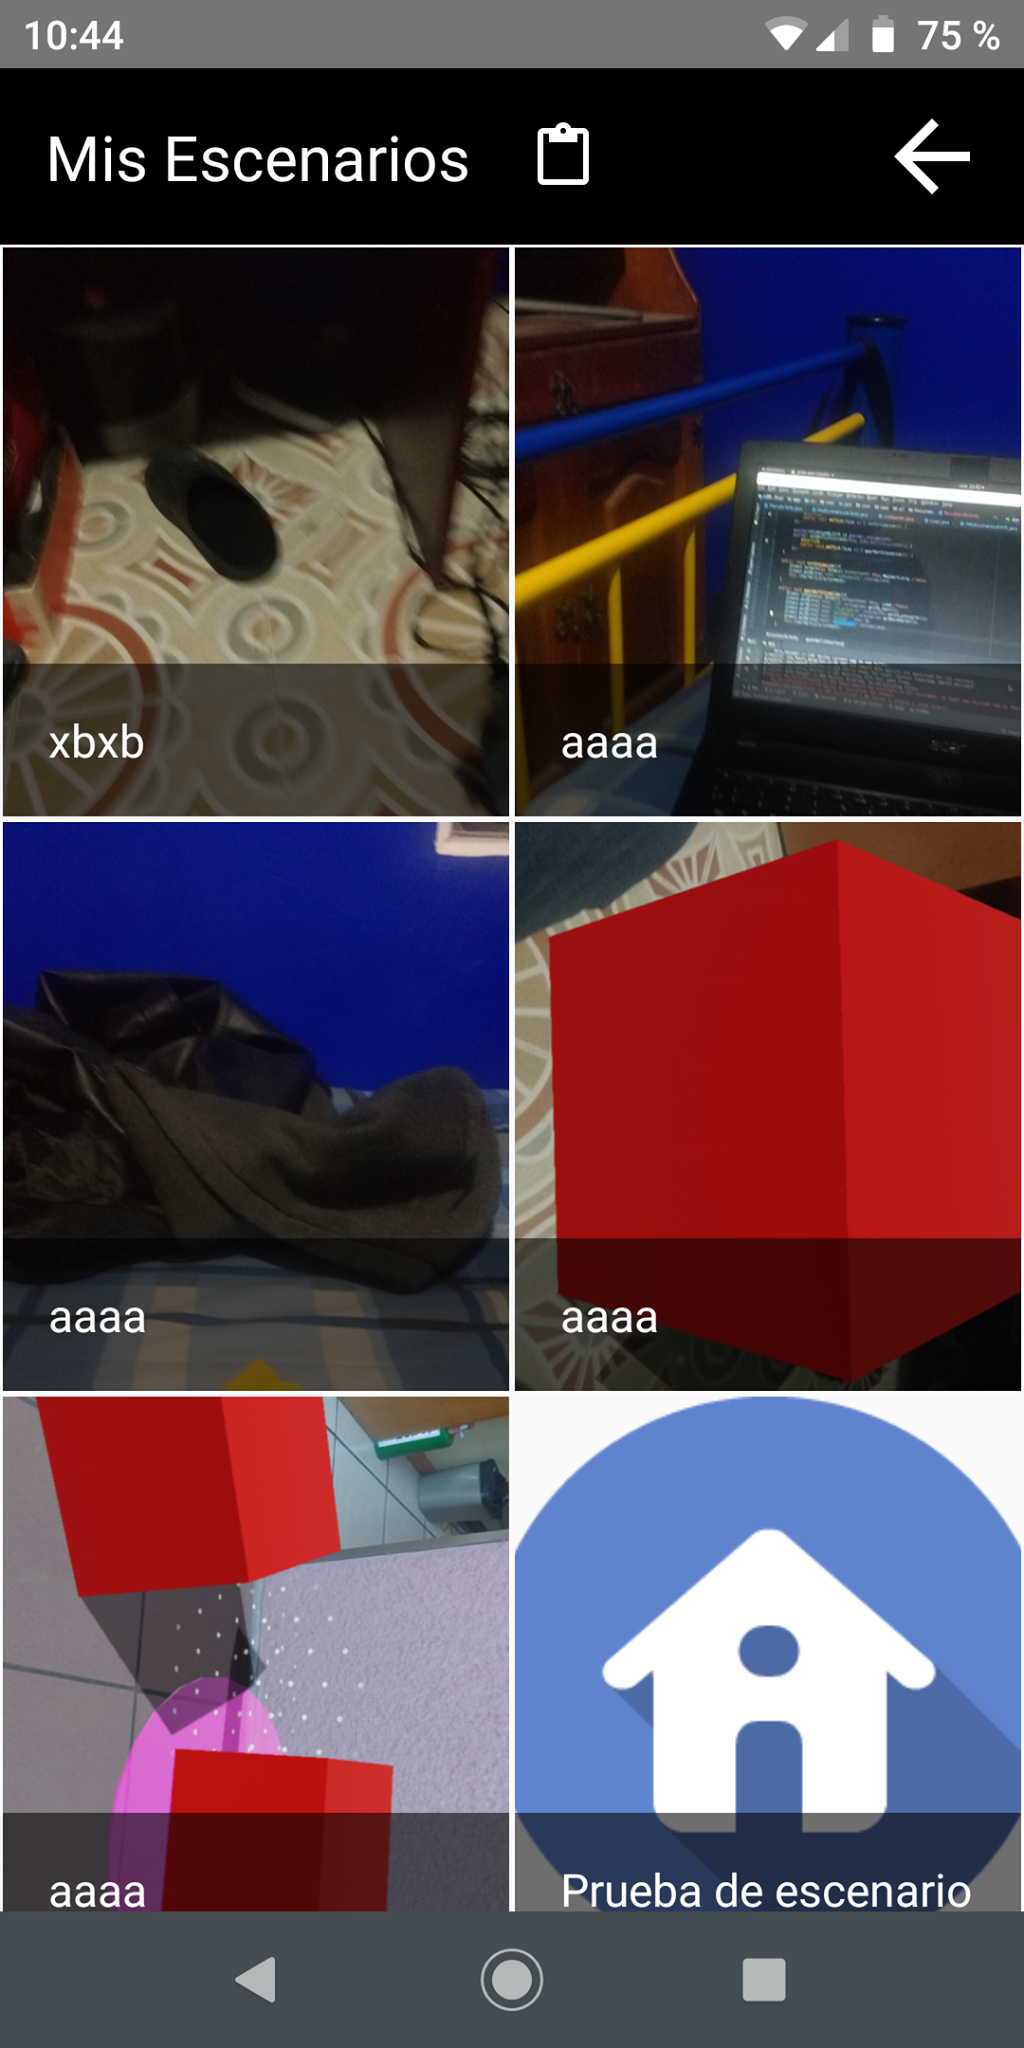
\includegraphics[width=4cm,height=8cm]{imagenes/desarrollo/app/scenarios.png}
		\caption{Mueble agregado a escena.}
		\label{fig:appfurn}
	\end{minipage}\hfill
\end{figure}

Las mejoras de usabilidad de la aplicación realizadas fueron las siguientes:
\begin{itemize}
	\item Cuando un mueble es seleccionado se muestra una marca debajo de él para identificarlo
	\item La pantalla de cámara la definimos en modo horizontal para que mostrara un mejor panorama de la escena.
	\item Cambiamos el aspecto de la barra de navegación de la aplicación a un diseño minimalista.
	\item En la esquina inferior izquierda se muestra el presupuesto definido al principio, el cual irá bajando o disminuyendo, dependiendo de los muebles que se agreguen o eliminen.
	\item Para posicionar un mueble tras seleccionarlo del menú omitimos el punto de referencia, en su lugar el usuario debe tocar la pantalla en el lugar donde desee posicionar el mueble.
\end{itemize}

\subsection{Resultados}
Al término de esta iteración obtuvimos una aplicación que:
\begin{itemize}
	\item Implementa la realidad aumentada
	\item Desarrolla y almacena propuestas de diseño de interiores (escenarios)
	\item Almacena modelos de muebles en la nube
	\item Gestiona proyectos para clientes
	\item Genera cotizaciones de las propuestas desarrolladas
\end{itemize}

El proceso de diseño de interiores cambia al usar la aplicación, en la figura 4.66 podemos ver el modelado de este nuevo proceso.
\begin{figure}[!htbp]
	\centering
	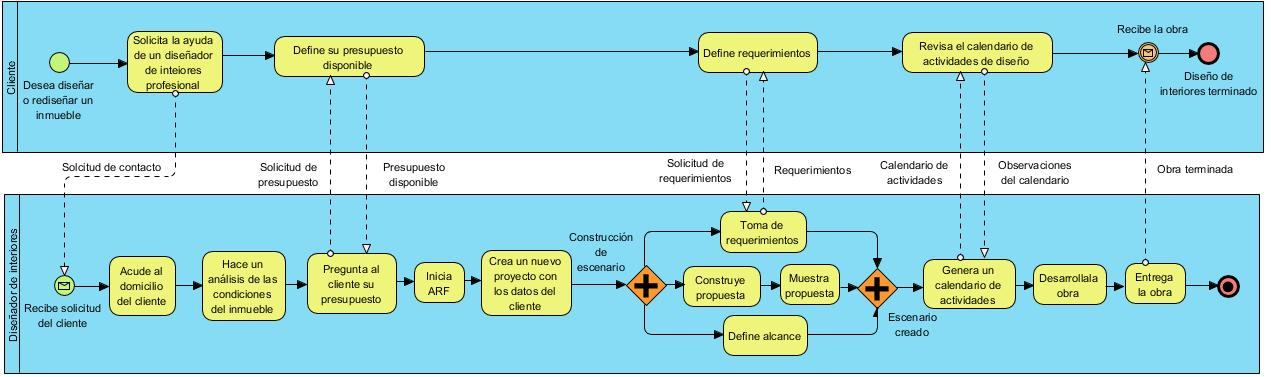
\includegraphics[width=20cm,angle=270,origin=c]{imagenes/desarrollo/diagramas/NPMN_FINAL_ID.jpg}
	\caption{Modelo del proceso de diseño de interiores usando ARF.}
	\label{fig:bpmnarf}
\end{figure}
\clearpage